\documentclass[a4paper,11pt]{mscLiterature}
%
\mscDepartment{Delft Center for Systems and Control}
\mscFaculty{Mechanical, Maritime and Materials Engineering}
\mscName{Thijs Ramakers, B.Sc}
\mscDate{\today}
\mscTitle{Speeding up on-line Reinforcement Learning using model-learning techniques} 
\mscSubTitle{Literature survey}
\mscKeyWords{literature, msc, subject}

\mscReaderOne{prof. R. Babuska}
\mscReaderTwo{dr. G. Lopes}
\mscReaderThree{MSc. E. Schuitema}
%\mscReaderFour{}
%
\setThesisInfo
%
\begin{document}
%
%============================= Front matter ========================================
\frontmatter %
%
% Make a hell of a lot of title pages
    \maketitle
%
% Abstract
    \nonumchap{Abstract}

		% Presentation Abstract
%Reinforcement Learning (RL) is a popular learning method. Learning is done by an agent that chooses actions and learns by observing state transitions and receiving reward for those transitions. Different basic solution methods exist that are capable of solving a RL task. Some of these methods rely on the availability of a model of the system, some learn without an explicit model and a third class builds a model during the learning process. These solution methods have all proven to be applicable, but only to relatively simple problems. In many applications however, large continuous state-spaces lead to a problem known as the curse of dimensionality. For these problems, learning becomes very slow or even impossible. An example of such a difficult learning task is learning a humanoid robot to walk. The robot learns from direct interaction with the environment, which is called on-line learning. The large number of continuous variables makes the application of RL a big challenge for such problems. 
%In this presentation model-learning methods for systems with large, continuous state-spaces will be discussed. The focus will be on dealing with continuous variables, storing the learned model efficiently and increasing the learning speed.

Reinforcement Learning (RL) is a popular learning paradigm. The learning process consists of an agent that chooses 	actions and learns from observing state transitions and receiving reward for those transitions. Different types of solution methods exist that are capable of solving a RL task. Some of these methods rely on the availability of a model of the system, some learn without an explicit model and a third class builds a model during the learning process. These solution methods have all proven to be applicable, but only to relatively simple problems. In many applications however, large continuous state-spaces lead to a problem known as the curse of dimensionality. For these problems, learning becomes very slow or even impossible. This survey explores how model-learning methods, which build a approximate model during the learning process, can be used to speed up the learning process in such cases. Different ways of approximating the value function and the transition model are reviewed. A two-legged, humanoid robot is presented as a challenging test case for these methods. 


   
    
    
    \cleardoublepage
%
% table of contents, (\toc of \toclof of \tocloflot )
    %\tocloflot
    \toc
%%
%% Nomenclature
%%    \nomenclature{$y$}{Description 2}%
%%		\nomenclature{$y$}{Description 2a}%
%		\lsymb{$L$}{Description 3}%
%		\gsymb{$\gamma$}{Discount factor}%
%    
%    \printnomencl %

% Acronyms
    \nonumchap{Acronyms} %
    %
    \begin{acronym}[XXXXXX]% Note: replace XXXXX by the longest acronym in your list.
				\acro{DBN}{Dynamic Bayesian Network}
 				\acro{DP}{Dynamic Programming}
 				\acro{KNN}{$K$-Nearest Neighbor}
 				\acro{LLR}{Local Linear Regression}
				\acro{MC}{Monte Carlo}
				\acro{MDP}{Markov Decision Process}
				\acro{MSE}{Mean Squared Error}
				\acro{NN}{Neural Network}
				\acro{POMDP}{Partially Observable Markov Decision Process}
				\acro{RBF}{Radial Basis Function}
				\acro{RL}{Reinforcement Learning}
				\acro{TD}{Temporal Difference}
				\acro{WLR}{Weighted Linear Regression}
		\end{acronym}%
    %
    \cleardoublepage%
%
% Index
    \printindex%
    \cleardoublepage%
%
%============================= Main matter =========================================
%
\mainmatter
%
\chapter{Introduction} \label{chap:introduction}

Self-learning systems are an interesting and inspiring idea. When confronted with a highly complex system, a thorough analysis is no longer needed to build a satisfactory controller. Instead, the system will learn how to behave by itself. Whenever the dynamics of the system or the environment change, there is no need for re-tuning the original controller. Instead, the system will adapt itself to these new circumstances. If a dangerous task has to be accomplished in an unknown environment, human intervention is no longer needed. Instead, an autonomous robot can do the task without help from a supervisor. 

Learning controllers are closing the gap between humans and robots. From the moment a human being is born, he starts discovering, learning and adapting. A learning controller mimics this behavior. It interacts with the environment to learn a control policy that completes the task at hand. 

	In reinforcement learning (RL), the controller learns by receiving feedback in the form of a scalar reward signal. The objective of the learning controller is to maximize the cumulative reward gained over the course of an experiment. Learning algorithms exist that require no explicit model of the system, but only need to observe system's state transitions and the associated rewards. 
	
	RL has proven to be successful in solving various problems of different size and complexity. In many cases however, RL has great difficulty in solving the problem. For systems with many states and multiple actuators, the state-action space quickly becomes too large to be able to use simple tabular methods in the learning process. In on-line learning on real setups, the continuous nature of the states leads to approximation and convergence problems. Both problems eventually result in slow learning and possibly in not finding an optimal policy at all.
	
	Several methods exist that can be used to speed up learning. Faster learning means that a larger class of problems can be solved with reasonable learning time. This literature report contains a survey on the current state of RL algorithms and possible methods for speeding up the learning. The goal of the final thesis itself will be to learn a two-legged robot called 'Leo' (Figure \ref{fig:Leo}) to walk. Leo has actuators in his hip, knees and feet. The robot has got 7 actuators and 8 sensors measuring both angle and position. In view of this learning goal, we focus in this literature report on methods that do not require an a priori model, that can handle continuous state spaces and that can be used in an on-line setting.
	
	This survey is organized as follows. First an introduction to Reinforcement Learning is given in Chapter \ref{chap:RL}. In Chapter \ref{chap:solutionMethods} an overview is given of several solution methods to the RL problem. In Chapter \ref{chap:modelLearningTechniquesOnRealSystems} a selection of methods that can be used to implement RL in a real-world, on-line setting are described. Chapter \ref{chap:otherRLMethods} briefly introduces other classes of RL techniques. Finally in Chapter \ref{chap:conclusion} we conclude which methods are interesting to apply to the robot problem.
	
\begin{figure}[htbp]
	\centering
		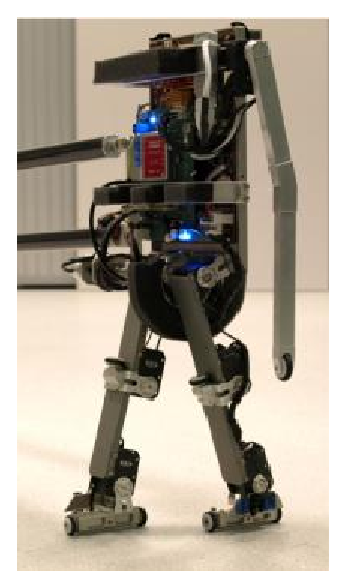
\includegraphics[width=200 pt]{img/leo1}
	\caption{The two-legged robot 'Leo'. The robot is actuated at the hip, the knees and the feet. The arm can be used to get up after the robot has fallen. The tubes on the left are attached to a central mounting point, so that the robot walks in circles.}
	\label{fig:Leo}
\end{figure}



    \cleardoublepage
%
% First Chapter: REINFORCEMENT LEARNING

    \chapter{Reinforcement Learning}\label{chap:RL}

    In this chapter, an introduction to Reinforcement Learning (RL) is given. First, the main ideas are presented with a short introduction of commonly used terms. Thereafter, a more formal description of the learning task is given and algorithms for solving the RL task are introduced. A nice overview of RL techniques can be found in \cite{SuttonBarto:98} and \cite{Kaelbling:96}.

        \section{Introduction}\label{sec:RLintroduction}
RL was inspired by human and animal learning. It is derived from the idea that past experience can be used for improving future behavior. The result of random actions in different situations is used to decide on actions in future situations that are similar. RL has a distinct 'trial and error' nature. Random actions are being tried, until the best action for a certain situation is found. Some frequently used terms are now introduced.

In RL learning is done by an \emph{agent} in close interaction with an \emph{environment} (Figure \ref{fig:RLframework}). The agent is the `learner' and the `decision maker'. It decides on what \emph{action} to take and evaluates the result of this action. The agent interacts with the environment to receive feedback in the form of a scalar \emph{reward} that indicates how 'good' the previous action was. In control applications, the agent will be represented by a computer program following a certain learning algorithm and the environment will be a system (either a real setup or a mathematical model) that reacts to the actions the agents takes. The environment also gives a reward signal to the agent. We are focusing on control applications in this survey, so we will assume that the interaction of the agent with the environment takes place at discrete time intervals. 
\begin{figure}[htbp]
	\centering
		\includegraphics[width=200 pt]{img/RLblockscheme}
	\caption{A schematic overview of the RL framework. The agent interacts with an environment and learns using a scalar reward.}
	\label{fig:RLframework}
\end{figure}
In many problems, a certain \emph{goal} state exists that the agent must try to reach. If this goal state is reached, the learning is stopped and the process is repeated. These separate experiments are called \emph{episodes} or \emph{trials}. The reward function can be defined in a number of ways. Usually, the reward will be positive if the goal is reached and negative or zero in all other cases. Note that the reward only qualifies the direct result of a certain action and not of the long-term effects of that action. The task of the agent will be to maximize the total (cumulated) reward, which requires the agent to asses the long-term effects of the action.

After a learning process, the agent `knows' how it can reach the goal. To be more precise, it knows what action it must take in every state in order to maximize the total reward. The set of rules that describe what action the agent will take in every state, is called the \emph{policy}.

So, in summary, the goal of a RL system is to find an optimal policy so that the total reward received during a trial is maximized. This is learned by an agent in close interaction with its environment.

\section{Markov Decision Process Framework} \label{sec:MDPframework}
In section \ref{sec:RLintroduction} we introduced the general idea behind RL and some important concepts used in RL. In this section, a more formal description of an RL problem will be given.

A requirement in RL is that the environment should have the Markov property. This means that if the current state is known, then the transition to the next state is independent of all previous states. However, this transition may still be deterministic or stochastic.

The state contains all the information that describes the system. In every state the agent has to make a decision based on an environment that has the Markov property, the learning task is therefore called an Markov Decision Process (MDP). When the state is not fully observable for the agent, such a task is called an Partially Observable Markov Decision Process (POMDP). 

Formally an MDP is a 4-tuple $(\mathcal{S},\mathcal{A},T,\rho)$. $\mathcal{S}$ is a finite set of states $s$ and $\mathcal{A}$ a finite set of actions $a$. $T:\mathcal{S}\times \mathcal{A}\times \mathcal{S} \rightarrow [0,1]$ is the state transition function which defines the probability of getting from state $s$ to $s'$ when action $a$ is taken. For deterministic environments this probability is either 0 or 1. $\rho:\mathcal{S}\times \mathcal{A}\times \mathcal{S} \rightarrow  \mathbb{R}$ defines the immediate reward $r$ for getting from state $s$ to $s'$ after taking action $a$. 

The policy is a mapping $\pi : \mathcal{S} \rightarrow \mathcal{A}$ that assigns an action to each state. The objective of the agent is to learn a policy that maximizes the expected total reward in the total experiment. The expected total reward $R_t$ after an action at time step $t$ is:
\begin{equation}\label{eqn:totalReward} 
	R_t = E\left\{ r_{t+1} + \gamma r_{t+2} + \gamma^2 r_{t+3} + ...\right\} = E\left\{ \sum_{t=0}^\infty\gamma^t r_{t+1} \right\}  \end{equation}
where $\gamma\in (0,1]$ is the discount factor. For problems with a finite time horizon, the upper bound of the summation is the final time step $t_\mathrm{f}$. The discount factor can be viewed in two different ways. The first view is purely mathematical. It makes sure that if the time horizon is infinite, the total reward converges to some finite value and will not go to infinity. The second view is more intuitive. By using a discount factor, rewards in the near future have an exponentially greater effect than rewards received in the far future. Because the discount factor is part of the learning task, the MDP is sometimes explicitly written as $(\mathcal{S},\mathcal{A},T,\rho,\gamma)$ to emphasize the discounting. 

\section{Value functions}
We can now proceed to assign a value to every state. The value of a state is the expected total reward in that state under a certain policy. This value function is therefore defined as:
\begin{equation}\label{eqn:valueFunctionDefinition} 
	V^\pi(s)=E^\pi \left\{ R_t \mid s_t=s  \right\}
\end{equation}
where $E^\pi\{\cdot\}$ is the expected value when following policy $\pi$. Because the goal of the agent is to learn which action is best in every state, it is also useful to define a value function that assigns a value to state-action pairs. To this end, the action-value function $Q(s,a)$ is defined:
\begin{equation}\label{eqn:actionValueFunctionDefinition} 
	Q^\pi(s,a)=E^\pi \left\{ R_t \mid s_t=s,a_t=a \right\}
\end{equation}
which also depends on the policy followed. Typically, for problems in which the agent knows how it can reach a certain state, the value function is convenient to use. For problems in which the agent does not know this, the action-value function can be used to explicitly store the reward for certain actions.



	\section{Optimal policy}
As mentioned before, the goal of the agent is to take actions which will result in the highest total reward. In other words, it has to find a policy $\pi$ that maximizes the value function $V^\pi(s)$ (or equivalently, $Q^\pi(s,a)$). This policy, which is better than all other policies, is called the optimal policy $\pi^*$. The value function that belongs to this policy is the optimal value function $V^*(s)$ and is defined as:
\begin{equation}\label{eqn:optimalValueFunction}
	V^*=\max_{\pi} V^\pi(s)
\end{equation}
The optimal policy has an optimal action-value function $Q^*(s,a)$:
\begin{equation}\label{eqn:optimalActionValueFunction} 
	Q^*(s,a) = \max_{\pi} Q^\pi(s,a) 
\end{equation}
which can also be written in terms of the optimal value function:
\begin{equation}
	Q^*(s,a) = E \left\{ r_{t+1} + \gamma V^* (s_{t+1}) \mid s_t=s,a_t=a \right\} 
\end{equation}
So, if the optimal (action-)value function is known, the optimal policy is the argument that maximizes \eqref{eqn:optimalValueFunction} or \eqref{eqn:optimalActionValueFunction}:
\begin{equation}\label{eqn:optimalPolicy}
	\pi^* = \arg\max_a Q^*(s,a) = \arg\max_a E \left\{ r_{t+1} + \gamma V^* (s_{t+1}) \mid s_t=s,a_t=a \right\} 
\end{equation}
Because this policy selects the action for which the (action-)value function is maximum, this policy is called a greedy policy.

Important for a large number of solution techniques are the so called Bellman equations. For the value function, these can be written as:
\begin{equation}\label{eqn:bellmanEquations}
\begin{aligned}
	V^\pi(s) &= E^\pi \left\{ \sum_{t=0}^{\infty}\gamma^t r_{t+1} \mid s_t=s \right\} \\
	& = E^\pi \left\{ r_{t+1} + \gamma\sum_{t=0}^{\infty}\gamma^t r_{t+2} \mid s_t = s \right\} \\
	& = E^\pi \left\{ r_{t+1} + \gamma V^\pi(s') \mid s_t = s, s_{t+1} = s' \right\} \\
	& = \sum_{s'} T(s,a,s') \left[ \rho(s,a,s') +\gamma V^\pi(s') \right]
\end{aligned}
\end{equation}
Recall that $T(s,a,s')$ is the transition probability from $s$ to $s'$ under action $a$ and $\rho(s,a,s')$ is the scalar reward for that transition. Using \eqnref{eqn:optimalValueFunction} we can derive the Bellman optimality equation for the value function:
\begin{equation}\label{eqn:bellmanOptimalityEquationStateValues}
	V^*(s) = \max_{a} \sum_{s'} T(s,a,s') \left[ \rho(s,a,s') +\gamma V^\pi(s') \right]
\end{equation}
And the equivalent Bellman optimality equation for the action-value function:
\begin{equation}\label{eqn:bellmanOptimalityEquationActionStateValues}
	Q^*(s) = \sum_{s'} T(s,a,s') \left[ \rho(s,a,s') +\gamma \max_{a'}Q^*(s',a') \right]
\end{equation}


\section{Conclusion}
In this chapter, we discussed the RL framework. Learning is done by an agent in close interaction with an environment. A scalar reward that is given for a state transition is the only information available to the agent for learning. The learning goal is to determine an optimal policy that leads to the highest long-term reward. An important tool for determining which action to take in which state is the value function. This indicates the expected long-term reward for a certain state or state-action pair. 
%The solution methods presented in the next chapter are all different ways of deriving a value function and using it to determine a policy. 













%Second Chapter: SOLUTION METHODS

\chapter{Solution methods}\label{chap:solutionMethods}
Several methods for solving RL problems exist. 'Solving' in a RL context means computing the optimal policy, which is generally derived from the optimal (action-)value function. The methods can be divided into three different types: model-based, model-free and model-learning methods. Model-based assumes there is a complete model of the environment available. Model-free methods start with no knowledge of the environment at all and learn from interaction with the environment. Model-learning methods also start with no a priori knowledge, but build a model while learning.

			\section{Model-based methods}\label{sec:modelBasedSolutionMethods}
			Model-based RL methods assume that the MDP is completely known and available to the agent. Not only is the state fully observable by the agent, also the state transition function $T$ and reward function $\rho$ are known. This means that the agent has a perfect model of the environment and its dynamics. The agent can calculate for every state the possible next states and their rewards. The Bellman optimality equations \eqnref{eqn:bellmanOptimalityEquationStateValues} and \eqnref{eqn:bellmanOptimalityEquationActionStateValues} lead to a system of equations with only $V^*(s)$ and $Q^*(s,a)$ as unknown variables and can therefore be solved. The need for a perfect model and the computational effort needed to solve these equations, makes the practical usability for these methods limited. However, these algorithms form the base of other methods. These model-based solution techniques are called Dynamic Programming (DP) \cite{Bellman:57}.
			
			\subsection{Policy iteration}
			Policy iteration uses two alternating steps: policy evaluation and policy improvement. The algorithm starts with a random initial policy $\pi_0$. The policy is used to obtain a first estimate of the value function $V_0(s)$ using Bellman equation \eqnref{eqn:bellmanEquations} for $\pi_0$ (the policy evaluation step). The obtained value function is used to compute a new policy $\pi_1$ using \eqnref{eqn:optimalPolicy} (the policy improvement step). This procedure is repeated until convergence is reached. Policy iteration is guaranteed to converge to the optimal value function and optimal policy. For episodic tasks, policy iteration converges in a finite number of steps.
			
			\subsection{Value iteration}
			Value iteration is a special case of policy iteration. It avoids the computationally heavy policy evaluation step. Instead of waiting for convergence to $V^*$, the policy evaluation is stopped after one step. The policy improvement step is the same as in policy iteration.
						
			\section{Model-free methods}\label{sec:modelFreeSolutionMethods}
		The methods presented in \ref{sec:modelBasedSolutionMethods} for solving RL problems, assume that a full model of the environment is available. In practice, this rarely is the case. Solution methods that do not need an explicit model of the environment are Monte Carlo and Temporal Difference methods. These solution methods rely on interaction with the environment only. Model-free methods are useful in practical problems where a model is either absent or very complex. Model-free learning methods that learn from interaction with the environment are also known as \emph{on-line} learning methods. Opposed to model-based methods which are also known as \emph{off-line} methods.
		
		\subsection{Monte Carlo methods}
		Monte Carlo (MC) methods are based on experience divided in episodes. Learning (i.e. updating the value function and policy) is done after an episode is completed. Monte Carlo methods work as follows: first an initial policy and (action-)value function are randomly generated. An episode is then carried out using the initial policy and all rewards are stored. After an episode has ended, every (action-)state that has been visited is updated using the average returns for that particular (action-)state. The policy is then updated and the whole process is repeated. 
		
		An important aspect of MC methods (in fact, of all model-free methods) is to make sure that all states are visited. All states must be frequently visited to guarantee convergence of the value function. This problem of sufficient \emph{exploration} is dealt with in section \ref{sec:exploration}.
		
		\subsection{Temporal Difference methods}\label{sec:TDmethods}
		MC methods, learn in an episode-by-episode way. Temporal difference (TD) methods on the other hand, learn in a step-by-step way. At every time step $t$, the agent takes an action for which it receives an immediate reward. At every time step the value function is updated according to:
		\begin{equation}
				V(s_t) \leftarrow (1-\alpha_t)V(s_t) + \alpha_t \left( r_{t+1} + \gamma V(s_{t+1}) \right)
		\end{equation}
		with $\alpha_t$ the learning rate at time step $t$. The learning rate indicates how strong new experience influences the estimate of the value function. A frequently used notation for TD algorithms is:
		\begin{equation}\label{eqn:TDbasic}
				V(s_t) \leftarrow V(s_t) + \alpha_t \delta_t
		\end{equation}
		with $\delta_t =  r_{t+1} + \gamma V(s_{t+1}) - V(s_t)$ the so-called TD-error. 
		
		\eqnref{eqn:TDbasic} shows TD in its most simple form. An algorithm using this update rule is called 1-step TD. As the name suggests, only rewards received at $t+1$ are used to update $V(s_t)$. It seems reasonable to also use $r_{t+2}$ to update $V(s_t)$. So, rewards further away in the future should be used to update a current value, but not as much as immediate rewards. The problem of how to use future rewards is called the \emph{credit assignment problem}. A basic way of using future rewards, is to incorporate \emph{eligibility traces} which will be discussed in the next section.
		
		\subsubsection{Eligibility traces}
				Eligibility traces indicate which states preceded the current state and are therefore eligible for change. Every state is assigned an extra variable called the eligibility trace $e_t(s)$. At every time step the eligibility traces decays with a factor $\gamma\lambda$ to make future states less dependent on the current state. $\lambda \in [0,1]$ is called the \emph{trace-decay parameter}. Different implementations exist, some of which are known to suffer from convergence problems. Here we introduce \emph{replacing traces}. At every time step, the trace is changed as follows:
				\begin{equation}
				e_t(s) = \left\{ \begin{array}{cc} \gamma\lambda e_{t-1}(s), & s\neq s_t \\ 1, & s=s_t \end{array} \right.
				\end{equation}
				The new update rule now becomes:
				\begin{equation}\label{eqn:TDeligibilityTraces}
					V(s_t) \leftarrow V(s_t) + \alpha_t \delta_t e_t(s_t)
				\end{equation}
				We notice the effect of choosing $\lambda$ either 0 or 1. $\lambda=0$ is the same as 1-step TD learning. When using $\lambda=1$ all the rewards received in an episode are used to update a value. So this is effectively the same as MC learning. So eligibility traces are bridging the gap between MC methods and 1-step TD methods. Because of the importance of the value of $\lambda$, a frequently used notation for TD with eligibility traces is TD($\lambda$).
		
	\subsection{TD implementations}		
	We will now discuss three important implementations of TD. All these methods can use eligibility traces, although for some a minor adjustment is needed.
	
		\paragraph{SARSA}
		SARSA \cite{RummeryNiranjan:94} uses $Q(s,a)$-values instead of $V(s)$-values for learning. As mentioned before, using state-action values is more convenient for control applications than storing state values only. It uses the same update rule as \eqnref{eqn:TDbasic}, but now with the state-action value function. Therefore the 1-step SARSA update rule is:
		\begin{equation}\label{eqn:SARSAbasic}
				Q(s_t,a_t) \leftarrow Q(s_t,a_t) + \alpha_t \delta_t
		\end{equation}
		with $\delta_t =  r_{t+1} + \gamma Q(s_{k+1},a_{k+1}) - Q(s_t,a_t)$. The update rule uses five values ($s_t,a_t,r_{t+1},s_{k+1},a_{k+1}$) which is the reason for the algorithm's name. To use eligibility traces with SARSA, one adjustment has to be made: the traces $e(s,a)$ should be associated with state-action pairs instead of states only. The new update rule now becomes:
		\begin{equation}\label{eqn:SARSAeligibilityTraces}
				Q(s_t,a_t) \leftarrow Q(s_t,a_t) + \alpha_t \delta_t e_t(s_t,a_t)
		\end{equation}
		When SARSA is used with eligibility traces, the resulting algorithm is commonly written as SARSA($\lambda$).

		\paragraph{Q-learning}
		As the name suggests, Q-learning \cite{WatkinsDayan:92} is also a TD method that estimates the action-value function $Q(s,a)$. As opposed to SARSA which is \emph{on-policy}, Q-learning is an \emph{off-policy} algorithm as it learns state-action values that are not necessarily on the policy that is followed. The Q-learning algorithm uses the following update rule:
		\begin{equation}
			Q(s_t,a_t) \leftarrow Q(s_t,a_t) + \alpha (r_{t+1} + \gamma\max_a Q(s_{t+1},a)-Q(s_t,a_t))
		\end{equation}
		Using eligibility traces with Q-learning requires one extra adjustment compared to using eligibility traces with SARSA. Since Q-learning is off-policy, state-action pairs should only be changed if they are followed by a greedy action. Whenever an explorative action is taken, the trace is reset to zero. This can be summarized as follows:
\begin{equation}
	\textrm{if a greedy action was taken:} \quad e_t(s,a) =
	\left\{
	\begin{array}{ll}
	1, & s = s_t, a = a_t   \\
	\gamma\lambda e_{t-1}(s,a), & \textrm{elsewhere}
	\end{array}
	\right.
\end{equation}
\begin{equation}
	\textrm{if an explorative action was taken:} \quad e_t(s,a) =
	\left\{
	\begin{array}{ll}
	1, & s = s_t, a = a_t   \\
	0, & \textrm{elsewhere}
	\end{array}
	\right.
\end{equation}
		The update rule for the Q-learning algorithm now becomes:
		\begin{equation}
			Q_{t+1}(s,a) \leftarrow Q_k(s,a) + \alpha\delta_t e_t(s,a)
		\end{equation}
		Q-learning with eligibility traces is written as Q($\lambda$)-learning.
		
		\paragraph{Actor-critic}
		Methods that store value functions and policies separately are called actor-critic methods. As opposed to methods that derive a policy from the action-value function. The term 'actor' refers to the policy (which action should be taken?). The term 'critic' refers to the value function (how good is the current state?). Updating both the policy and value function is done using TD methods and use an update rule such as \eqnref{eqn:TDbasic}.
			
		\section{Model-learning methods} \label{sec:modelLearningMethods}
		We have introduced two types of RL methods. One based on the availability of an accurate model and one based on the situation in which no model is present. Now, consider that there is initially no model present. For these cases, one would use a model-free method. Two questions arise: could we use past experience to estimate a model during learning? And can we then use this model to speed up the learning process? In this section we introduce model-learning methods that use experience to build a model upon which model-based techniques can be applied. 
		
		\cite{Sutton:90} argues there are great similarities between model-based and model-free RL methods. Different methods could therefore be combined, which he calls: integrating \emph{learning}, \emph{planning} and \emph{acting} (see Figure \ref{fig:integratingLearningPlanningActing}). Where the term planning is used to refer to off-line, model-based techniques (DP) and learning to on-line, model-free techniques (MC, TD). Acting refers to on-line learning situations in which interaction with the environment (controlling actuators, reading sensor data) consumes an important part of every time step. Sutton introduces \emph{Dyna-Q} and \emph{Dyna-PI} as methods to combine planning with learning. The general class of \emph{Dyna} algorithms will be discussed next.		
\begin{figure}[htbp]
	\centering
		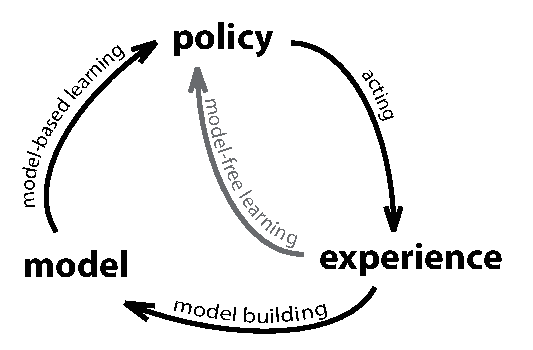
\includegraphics[width=300 pt]{img/LearningPlanningActing}
	\caption{Integrating learning, planning and acting in the Dyna framework.}
	\label{fig:integratingLearningPlanningActing}
\end{figure}
				
	\subsection{Dyna} \label{sec:dyna}
	Dyna is a general term that is used for a class of algorithms that combine learning from real experiences with learning from simulated experiences generated using a (learned) model. The difference lies in the algorithms and the type of value function that is used. For example, Dyna-Q and Dyna-PI use Q-learning and policy iteration as learning algorithms respectively.
	
	The idea behind Dyna algorithms is as follows: After initializing a (random) model and value function, an action is taken and the next state and reward are received. The update rule from any model-free learning method is then applied and the model is updated using the experience gained. Thereafter, model-based techniques are applied to the learned model. The number of iterations for this step can be either fixed or variable depending on the problem. For instance, in an on-line setting the time left in a particular sampling interval can be used for model-based learning. The ratio between real world and simulated samples can therefore vary. In short, the agent interacts with the system and the learned model alternatively (Figure \ref{fig:DynaFramework}).
	\begin{figure}[htbp]
	\centering
		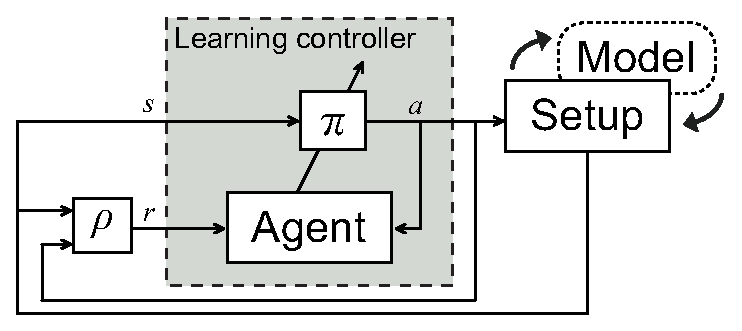
\includegraphics[width=300 pt]{img/DynaFramework}
	\caption{Schematic overview of the Dyna algorithm, which switches between interaction with the real system and its model.}
	\label{fig:DynaFramework}
\end{figure}

	To have the most profit of using building a model, it is important that the model is a good approximation of the real system. The model has to be accurate for the total state-space. \cite{Schmidhuber:91} introduces so-called curious model-building systems that include a confidence measure. Schmidhuber introduces the terms 'curiosity' and 'boredom' for part of the state-space that need to be visited or are already modeled accurately.
	
	A variation on Dyna is \emph{experience replay} \cite{Lin:92}. Instead of learning a model, past transitions are simply stored. These past experiences are then used repeatedly by the algorithm.
	
	\subsubsection{Prioritized Sweeping}
	In Dyna, the states that are selected for planning can be chosen randomly. However, this seems not to be the best choice. Especially in large state-action spaces or early in the learning process, a lot of states will not contain any information regarding the goal state (because the goal has never been reached and therefore its value will still be zero). Therefore, it makes sense to concentrate the computational effort to areas of the state-action space where it is most effective. In other words, we want to prioritize important states in some way. 
	
	\cite{MooreAtkeson:93} and \cite{PengWilliams:93} independently developed strategies to speed up the planning in Dyna by introducing a priority queue. Moore and Atkeson focused mainly on explicitly learning the state-transition model with all its transition probabilities. They named their method \emph{Prioritized Sweeping} (PS). Peng and Williams used Dyna-Q as learning algorithm, and also used a priority queue to speed up learning. They named their method \emph{Queue-Dyna}. In both approaches, a queue is maintained that determines the order in which states should be updated during planning. The two methods are almost identical. They only differ in which states they allow onto the priority queue. Where PS allows all predecessors which have a predicted change on the queue, Queue-Dyna allows only states that have a change greater than some threshold value. As mentioned, these differences are small and probably only influence memory usage in practice, but not learning speed. 
	
	The importance of a state that determines its place in the queue can be determined in several ways. The general way is to take the absolute value of the TD-error $\delta_t$. The larger this error, the more the value for a certain state has changed and thus the more influence it has on the total value function. 
	
	Most of the articles dealing with PS techniques report improved performance compared to standard Dyna \cite{MooreAtkeson:93}, \cite{PengWilliams:93}, \cite{Rayner:07}, and also \cite{Wingate:05}. However, it has been reported \cite{Grzes:08} that PS can also lead to worse performance for some specific tasks. In this task a maze has to be navigated towards a goal. Along the way, several flags can be 'set'. Setting a flag is a sub-goal and gives the agent a higher reward when the ultimate goal is reached thereafter. When not all flags are set, the goal can be reached, but the total reward is not maximum. Grze\'{s} argues that this effect is due to the many sub-optimal solutions for the task. PS would lead to insufficient exploration in such cases. However, it is not clear how the type of exploration, the exploration rate and learning rate influence this effect. 
	
	\subsection{How can model-learning speed up learning?}
	The reason that one would use model-learning methods instead of model-free methods is that the learning speed can be increased. Some reasons that explain why building a model increases learning speed are given.
	
	Probably the most important reason, is that real-world experiences are relatively rare in on-line learning. So the experiences that are available should be used as effectively as possible. With model-free learning, experiences are used only once (when updating the value function). In model-learning, the experiences are not only used in the update-rule, but also for building a model. So, for every model-based update, past experiences are used again. So experiences are used more efficiently.
	
	Another reason why model-learning methods are useful, is that a larger part of the state-space can be updated. Not only the limited number of states that are visited by the agent during a trial can be updated. The model makes it possible to update every other state. So the model enables the agent to update a larger part of the state-space.
	
	A last advantage of using model-learning methods in on-line learning, compared to model-free methods, is the use of the sampling interval. In model-free learning, every sampling interval is used for only one update of the value function. The time needed for the update is typically less than the sampling time, so a part of the sampling interval is left unused. The unused time could be reduced by choosing a higher sampling time. However, choosing a higher sampling time can be either not possible (because it takes time to use the actuators and read sensor data) or not useful (because the system's state has not significantly changed after a very short time). In model-learning, the total sampling interval can be used. The remaining sampling time (which would otherwise be left unused) can be filled with off-line updates.
	

	
	
	\section{Issues with solving RL problems} \label{sec:issuesWithSolvingRLProblems}
	The RL framework and several methods for solving RL problems were introduced in Chapter \ref{chap:RL} and \ref{chap:solutionMethods}. The methods discussed have all been successfully applied to RL tasks (see \cite{SuttonBarto:98} for multiple examples). However, there are several issues to deal with when solving RL problems. These issues are particularly important for real-world, on-line application of RL in which we have to compute the optimal policy for large, continuous state-spaces. Some of the most important issues will be discussed in this section.
	
	\subsection{Sufficient exploration}\label{sec:exploration}
	A problem that exists especially in model-free methods is the dilemma of exploitation versus exploration. The agent should use (exploit) experience gained to optimize the current policy. On the other hand, the agent should maintain its search in the state-space (explore) to find possible better policies. In fact most proofs of the policy converging to the optimal policy, only hold when the total state-space is constantly visited. Different strategies exist that describe how the agent should explore the state-space.
	
	\paragraph{$\epsilon$-greedy}
	The most straightforward exploration method is $\epsilon$-greedy. The exploration rate $\epsilon$ gives the chance of choosing an explorative action, instead of the current optimal (greedy) action. The exploration rate does not have to be constant during the learning task, but can be gradually decreased allowing less explorative actions as learning proceeds.
	
	\paragraph{Max-Boltzmann}
	Another approach is to select action $a$ in state $s$ with a probability $p(a|s)$. The probability distribution is given according to the Boltzmann distribution:
	\begin{equation}
		p(a|s) = \frac{e^{Q(s,a)/\tau}}{\sum_{a'\in \mathcal{A}}{e^{Q(s,a')/\tau}}}
	\end{equation}
	where $\tau$ is the temperature parameter. The larger this parameter, the larger the probability of choosing an explorative action. This parameter may also be decreased during the learning process, to decrease exploration.
		
	\paragraph{Directed exploration}
	$\epsilon$-greedy and Max-Boltzmann exploration are methods that select random explorative actions. A different group of exploration strategies is called directed exploration. As the name suggests, these methods direct the agent to search in a certain direction, that could possibly be an interesting part of the state-space. We mention a few possible ways of determining the probability distribution. A way to include a 'direction' is to add an exploration bonus to the estimated action-value function (\cite{Bakker:06}) for certain actions.
	
	The first way is counter based. An extra variable is included, that counts the number of times a certain action has been taken in some state. Rarely taken actions will be chosen with a higher probability than frequently chosen actions. This method is therefore called \emph{frequency based} exploration. 
	
	A second way that is also counter based, is \emph{recency based} exploration. Actions that have been taken long ago, will be more likely to be chosen than recently selected actions. This is also a way to make sure that all actions are chosen during the learning task.
	
	\cite{vanAstBabuska:06} introduce an exploration method called \emph{dynamic} exploration. This method is inspired by the idea that in real-world problems, often long sequences of the same action have to be taken. Therefore, the action that was chosen in the previous time step has a higher probability to be chosen again.
	
	\subsection{Curse of dimensionality}
	A second problem faced by RL algorithms is a problem called the \emph{curse of dimensionality}. If we consider a tabular representation of the state and action variables, the memory and computational time needed by the algorithm increase exponentially with the dimension of the state-action space. Different approaches to deal with this problem have been developed, such as variable resolution discretization (see Section \ref{sec:discretization}) and function approximation (see Section \ref{sec:functionApproximation}). Despite the existing methods to deal with this problem, scaling up RL to high-dimensional tasks remains probably the greatest challenge faced by researchers. 	

	\subsubsection{Slow propagation of information}
	A problem that is closely related to the curse of dimensionality is the propagation of information through the state-space. At the beginning of the learning process, the value function does not yet contain any information on the goal state. Once the goal is found, this information has to propagate through the state-space. This propagation can consume a great amount of time, since the information has to be back-propagated through the entire state-space. 

	\subsection{Application on real setups} \label{sec:applicationOnRealSetups}
	A few problems that occur when RL is applied to real setups will be discussed briefly. The first important issue is continuous variables. Many interesting real setups have continuous state and action variables. The RL framework was defined for discrete states and actions. Several methods to deal with continuous variables have been developed (see Sections \ref{sec:discretization} and \ref{sec:functionApproximation}). A problem with using these techniques is that in most cases convergence cannot be guaranteed in all cases. 
	
	A second issue is sampling time limitations. When interacting with a real system, the sampling time dictates the time available to the algorithm to do computations. So the algorithm must work fast enough to be ready before the next action has to be taken. On the other hand, if the algorithm has finished before the end of the sampling interval, time is left to do more calculations which could lead to increased learning speed. 	
	
	The third issue is dealing with disturbances. The disturbances can be either deterministic or stochastic. The deterministic disturbances are due to external influences on the system. When we consider a walking robot for example, these disturbances could be due to the surface of the terrain, the influence of the wind or some load carried by the robot. The disturbances can also be more stochastic in nature. Stochastic disturbances are common when dealing with real systems (\cite{Mahadevan:96}). Models will never be able to fully describe the system and some random disturbances will always be present. Sensor noise is also an always present disturbance in real systems.
	
	\subsection{Convergence properties}
	So far we have not addressed the question whether or not the mentioned solutions indeed lead to the optimal policy. This is the problem of convergence (to the optimal solution). In this chapter, we have focused on RL in its most standard form: a discrete state-action space and exact tabular representations of the value functions. Proofs of convergence exist when these problems are solved using the solution methods mentioned in this chapter. 
	
	However, as we will see in Chapter \ref{chap:modelLearningTechniquesOnRealSystems}, in large discrete or continuous state-spaces this tabular approach is no longer feasible. Approximate solution methods have to be used to solve the RL problem. Convergence properties of tabular solution methods can not be transferred directly to approximate solutions. For some combinations of approximators and solution algorithms, convergence proofs still exist. For example \cite{Gordon:95} provides a proof of convergence for TD methods combined with a class of function approximators called 'averagers'. For many of the approximate solution methods however, such proofs do not exist. In these cases, solutions to the learning task may be sub-optimal or a solution may never be found at all. 
	
	RL is in general a heuristic field. Standard learning tasks are used to prove the usefulness of new algorithms and convergence proofs are frequently left behind. Although successful applications of approximate RL methods are widely available, one has to be careful when applying them.

\section{Conclusion}
In this chapter, three different types of solution methods to the RL problem were presented. Model-based methods use an available model of the environment to iteratively calculate the optimal value function. Model-free methods are used in an on-line setting where no explicit model of the environment is available. A combination of these two lead to the model-learning class in which model-free and model-based learning techniques are combined. Different reasons were presented why model-learning techniques can improve learning speed compared to model-free methods. For the two-legged humanoid robot Leo, no a priori model is available, so model-learning methods seem to be the most promising for solving this learning problem.












\chapter{Model-learning techniques on real setups} \label{chap:modelLearningTechniquesOnRealSystems}
Up until now we have considered RL in its most basic form, using only discrete states and actions. In this chapter we shift our attention to solving real-world problems, such as the two-legged robot mentioned in the Chapter \ref{chap:introduction}. We have the following assumptions for such tasks. First, we have to deal with a continuous state-space. Second, an a priori model is not available and has to be approximated during on-line learning. Some issues with RL in real applications were already mentioned in Section \ref{sec:issuesWithSolvingRLProblems}. Here, we will discuss several methods to overcome these problems and to make learning as efficient and effective as possible.
%Second, no a priori knowledge is used. This means that, prior to the learning process, no model of the environment is available to the learning agent. Third, learning has to be done in an on-line setting by interaction of the system with the environment. 

%In this chapter we focus on model-learning techniques such as Dyna (Section \ref{sec:dyna}) in an on-line setting. 

	
	
\section{Value function approximation}\label{sec:ApproximatingTheValueFunction}
	Approximation of the value function is needed in cases where listing all possible state-action pairs in a table is either inconvenient or even impossible. In cases with a very high number of discrete states, listing them is inconvenient. But in tasks with continuous states, listing the states is simply impossible. Approximation or generalization are terms that are used to indicate that some sort of method of approximating the value function is used.
	
	\subsection{Discretization}\label{sec:discretization}
	The most straightforward way of approximating the (continuous) states is by discretizing the state-space. For these methods, the state-space is divided by a grid of some sort into a finite number of states. The resolution of the grid can be either constant, variable or dynamic. 
	\subsubsection{Constant resolution}
	Using a grid with some fixed resolution is the most simple form of discretization. The number of states is directly related to the resolution. The resolution is chosen a priori by the experimenter, such that it is not too high (which would result in a state-space that is too large to solve) and not too low (which would result in an agent that is not able to learn). 
	\subsubsection{Variable resolution}
	Using a constant resolution is not the best choice, as it assumes that all parts of the state-space are equally important. It seems reasonable that areas close to the goal (or that are important in some other way) need a finer resolution than states further away (or less important). Using a grid with a resolution that variates over the state-space, gives the experimenter more freedom in determining where the important parts of the state-space are. The experimenter should use its knowledge about the system and its goal to determine the grid. A possibility could be for example a logarithmically scaled grid, which has lots of states close to the goal and fewer states far away.
	\subsubsection{Dynamic resolution}
	Variable resolution techniques are interesting, but they require expert knowledge for determining the resolution of the grid. Therefore, dynamic resolution methods have been developed. In these methods, it is the algorithm itself that adapts the resolution during the learning process. To determine where to split grid cells, a splitting criterion has to be introduced. \cite{MunosMoore:01} suggest 'influence' or 'variance' as splitting criteria. A different well known dynamic resolution algorithm is the Parti-Game algorithm by \cite{MooreAtkeson:95}. A downside of variable resolution algorithms is that they are only applicable to off-line, model-based tasks. So they cannot be used in the on-line, model-learning tasks such as the one we are considering here.
	


	\subsection{Function approximation} \label{sec:functionApproximation}
	When dealing with real setups with continuous variables or problems with very large state spaces, using a tabular value function such as in Section \ref{sec:discretization} becomes impossible. Not only would the memory needed to store such a value function become very high, also solving the RL task would become impossible as the state-action space would be too large to explore within a reasonable time. For these tasks, a generalization technique known as Function Approximation (FA) has to be used. 
	
	In FA the value function is not represented by a table, but approximated by a parametric function $V_t(s)$ with parameter vector $\theta_t\in \mathbb{R}^n$ at time step $t$. The solution methods in Chapter \ref{chap:solutionMethods} are not applicable for this case, as we no longer have the possibility of making updates of states. We describe gradient descent methods to use FA in RL. Thereafter we discuss possible options for approximation functions. 
	
	\subsubsection{Gradient descent methods}
	As mentioned, table-based solution methods cannot be used with FA. Gradient descent methods have to used when the value function is approximated by a parametric function. These methods rely on minimizing the Mean Squared Error (MSE) between the real value function and the current estimate:
	\begin{equation}
		\textrm{MSE}(\theta_t) = \sum_{s\in \mathcal{S}} \left( V^\pi(s) - V_t(s)\right)^2
	\end{equation}
	We are searching for the (global) optimal parameter vector $\theta^*$ for which $\textrm{MSE}(\theta^*) \leq \textrm{MSE}(\theta)$ for all $\theta$. In general the $\textrm{MSE}(\theta^*)$ will not be exactly zero as the parametric function is an estimation of the real value function. The parameters vector can be adjusted using gradient information:
	\begin{equation}
	\begin{aligned}
		\theta_{t+1} &= \theta_t - \frac{1}{2}\alpha\nabla_{\theta_t}\left( V^\pi(s) - V_t(s) \right)^2 \\
		&= \theta_t + \alpha\left( V^\pi(s) - V_t(s) \right) \nabla_{\theta_t}V_t(s)
	\end{aligned}
	\end{equation}
	where $\alpha > 0$ denotes a step-size parameter and $\nabla_{\theta_t}$ the differential operator which gives a vector of partial derivatives. $V^\pi(s)$ is unknown, but we can use TD methods of section \ref{sec:TDmethods} to write:
	\begin{equation}\label{eqn:gradientDescentUpdateRule}
		\theta_{t+1} = \theta_t + \alpha \delta_t e_t
	\end{equation}
	with $\delta_t = t_{t+1} + \gamma V_t(s_{t+1}) - V_t(s_t)$ the TD-error and $e_t = \gamma\lambda e_{t-1} + \nabla_{\theta_t} V_t(s_t)$ a vector of eligibility traces (for each component of $\theta_t$). This is the most general form of the gradient descent method and can be easily rewritten for the action-value function. In the next sections, different types of approximation will be introduced.
	
	\subsection{Linear function approximation}
	A important class of approximators are function approximators that are linear in the parameter vector. For this class, the value function is approximated by a parameter vector $\theta_t$ and a feature vector $\phi_s \in \mathbb{R}^n$. The value function is approximated as:
	\begin{equation}
		V_t(s) \approx \theta_t^T \phi_s = \sum_{i=1}^n{\theta_t(i)\phi_s(i)}
	\end{equation}
	The big advantage of using a linear approximator, is that the gradient of $V_t(s)$ with respect to $\theta$ is simply:
	\begin{equation}
		\nabla_{\theta_t} V_t(s) = \phi_s
	\end{equation}
	So the update rule in \eqnref{eqn:gradientDescentUpdateRule} becomes very simple. Another advantage of linear approximators is that there exists one globally optimal parameter vector $\theta^*$. Due to the convexity of this optimization, we are guaranteed to converge to the global optimal parameter vector.
	
	The only remaining part, is to describe the feature vector $\phi_s$. Several options exist, that will be discussed next.
	
	\subsubsection{Tile coding}
	In tile coding (also known as Cerebellar Model Articulation Controller, or CMAC) the state-space is partitioned in a number of subsets, often by simply introducing a grid. Each partition is called a tiling. Each subset is called a tile and corresponds to a feature $\phi_s(i)$. The parameter vector indicates whether a state lies in tile $i$ ($\theta_t(i) = 1$) or not ($\theta_t(i) = 0$). The entire state-space is covered with multiple tilings, each with an small offset relative to each other. In this way, a small number of tiles can be used for a good generalization over the total state-space. 
	
	In this method, a tiling does not have to be divided using a rectangular grid. For example circular tiles could be used or in fact any shape could be used. The experimenter can use its knowledge of the system to choose a tiling that is most useful for the task at hand. Using a simple grid however, has the advantage of being easy to implement when used on a computer. 
	
	Another trick to keep memory demands low in high-dimensional spaces, is to neglect some dimensions completely or to use very coarse tiles. For many problems this leads to a much lower memory usage, but still reasonably good approximation.
	
	\cite{Sutton:96} and \cite{Boone:97} provide examples of successfully applying CMAC as function approximator in an on-line, model-free learning setting. 
	

	\subsubsection{Radial basis functions}
	In tile coding the parameter vector has binary entries. One could also think of choosing the parameter vector in the interval $[0,1]$, describing the degree to which a feature is present in a state. Radial Basis Functions (RBFs) can be seen as the continuous counterpart of tiles. The value of a RBF depends on the distance $r_i$ of the state to some center $c_i$, so $\phi_i(s,c_i) = \phi_i(\left\|s-c_i\right\|) = \phi_i(r_i)$.	Different choices for the feature vector can be made. The feature vector can be a thin plate spline function:
	\begin{equation}
		\phi(r_i) = r_i^2 \log(r_i)
	\end{equation}
	or a multi quadratic function:
	\begin{equation}
		\phi(r_i) = \sqrt{r_i^2 + \rho^2}
	\end{equation}
	with $\rho>0$. The most commonly used RBF is probably a Gaussian function:
	\begin{equation}
		\phi_i(r_i) = \textrm{exp} \left( -\frac{r_i}{2\sigma_i^2} \right)
	\end{equation}
	where $\sigma_i$ is the feature's width. RBFs are smooth and differentiable. The downside of using RBFs is that the computational complexity and tuning time increases, especially when the centers and widths of the features are varied over the state-space.
	
\subsection{Nonlinear function approximators}

\subsubsection{Neural networks}
The most common form of a nonlinear function approximator is the Neural Network (NN). The architecture of a neural network consists of several inputs, one or more outputs and one or more hidden layers. A network is trained by adapting the weights of the connections between the nodes in the network. NNs are used to approximate nonlinear functions and can be used for very large state-spaces (\cite{Gaskett:99}, \cite{RandlovAlstrom:98}, \cite{Riedmiller:05}).

 An example of how well NNs scale to large state-spaces is TD-gammon \cite{Tesauro:95}. TD-gammon is a neural network that learns to play the game of backgammon using RL techniques. TD-gammon learned itself to play the game at expert level. This is a great achievement since the game has approximately $10^{20}$ states.

Theoretically, a single-layer NN with sigmodial activation functions can approximate any continuous nonlinear function arbitrarily well, provided that the number of hidden neurons is sufficient. The number of neurons is a matter of trial and error. Too few neurons lead to a poor fit, while too many neurons may lead to overfitting. The number of hidden layers may also be increased to improve the approximation, but this leads to longer training times.

Training a NN means adjusting the weights to reduce the modeling error (the difference between the actual output and the modeled output). This results in a (nonlinear) optimization problem with respect to the weights. Solving such problems requires optimization algorithms, which we will not discuss in detail here.

In an on-line RL task, training a NN is done by the transitions observed by the agent. These transitions result in a set of training data, which increases in size during the learning process. 

\section{Learning the state transition model}
%	
%- Dynamic Bayes Network (DBN) ((Tadepally & Ok, 1996; Andre, Friedman & Parr, 1998; Guestrin et al., 2003).
%Guestrin, Hauskrecht and Kveton (2004))
%- Boutilier, Dearden and Goldszmidt (2000): Decision trees (Degris, Sigaud and Wuillemin (2006))
%- Lagondakis, Parr: support vector machines
%-Atkeson, 1993; Atkeson, Moore \& Schaal, 1997; Nouri \& Littman, 2006).

Model-learning techniques such as Dyna, learn a model of the environment. Learning a model means approximating (learning) the state transition function $T(s,a,s')$ and the reward function $R(s,a,s')$ from real-world interactions. Learning the model has to be done during learning and from a very limited set of data. In general, estimating the transition function is more difficult than the reward function, since the former can be probabilistic in nature. Different methods for learning a model exist. The methods can be divided into two types: eager learners and lazy learners. Eager learners adjust the model whenever a new experience is received. Lazy learners store past experiences and approximate a model when a query input is received. Lazy learning is therefore also known as memory-based learning.

\subsection{Tabular representation}
The most basic way of estimating a transition model is to count how often a certain transition has occurred for every state-action pair. The transition probability is then determined by the frequency of that particular transition. The reward function is estimated by observing the immediate reward for a certain transition. This information is simply stored in a tabular way. Therefore, the tabular approach can be seen as the most basic form of lazy learning. This method is only usable in small, discrete state-spaces. 

For continuous spaces, the exact same state will never be visited twice. Therefor, the continuous state-space has to be discretized to a reasonably low resolution. This is also called aggregating states, as multiple states are aggregated together. With this tabular approach, a better model can only be obtained by using a finer resolution and thus increasing the memory needed and decreasing the generalization. 

In surprisingly many experiments, the model is learned using this tabular approach. Even in tasks with continuous state-spaces. An example can be found in \cite{KuvayevSutton:96}, where the tabular representation of the model is used along with CMAC as function approximation. 

\subsection{Linear model}\label{sec:linearModel}
A linear model consists of a forward transition matrix $F \in \mathbb{R}^n \times \mathbb{R}^n$ and an expected reward vector $b \in \mathbb{R}^n$, such that $\phi_s' = F \phi_s$ and $r_{t+1} = b^T \phi_s$. $F$ and $b$ are updated using TD methods:
\begin{equation}
	\begin{aligned}
	F &\leftarrow F + \alpha(\phi_s'-F\phi_s)\phi_s^T \\
	b &\leftarrow b + \alpha(r_{t+1}-b^T\phi_s)\phi_s
	\end{aligned}
\end{equation}
with $\alpha$ the learning speed. This is essentially TD applied to the transition matrix and the reward vector. This eager learning method updates the model with every new experience. Section \ref{sec:PSwithFA} shows how this method can be combined with PS.


\subsection{K-nearest neighbor}
The $K$-Nearest Neighbor (KNN) method, is based on storing past input-output pairs (i.e., memory-based). Consider a set of $N$ input-output samples $(x_s,y_s)$. The model gives an approximate output $\hat{y}_q$ to a query input $x_q$. The approximation is calculated based a the $K$ nearest sample inputs in the memory according to some distance measure $d_s$ relative to the query input (see Figure \ref{fig:KNN}) and is therefore a local approximation method. The distance measure can be any (weighted) norm (\cite{Atkeson:97a}). Weighting can be used to weight important state variables more than others. The $K$ selected samples, are then used to approximate the output for the query input. In its most basic form, the KNN method simply averages over the $K$ output samples:
\begin{equation}
	\hat{y}_q = \frac{\sum_{s=1}^K {\frac{1}{d_s+\delta}}y_s}{\sum_{s=2}^K{\frac{1}{d_s+\delta}}}
\end{equation}
where a small constant $\delta$ is introduced to avoid division by zero. This methods works fast in one and two dimensional spaces. In high-dimensional spaces, the calculation of $d_s$ becomes computationally heavy.
\begin{figure}[htbp]
	\centering
		\includegraphics[width=200 pt]{img/KNN}
	\caption{2 dimensional representation of the KNN method. The dots represent the stored samples and the cross is the query point. The dark dots are the $K$ closest neighbors ($K=5$ is this example).}
	\label{fig:KNN}
\end{figure}
It is important to decide which past experiences should be stored. Storing all experienced transitions, would require large amounts of memory and a large amount of computational power. Storing only a small number of transitions would lead to an inaccurate model. Some sort of memory management is needed to determine which input-output pairs should be stored in order to get a good trade-off between model accuracy and computational demands.
 
 
% Lazy learning \cite{Aha:98}


\subsection{Local linear regression}
The basic KNN method can be extended by, instead of averaging, fitting a linear model to the $K$ input-output pairs. This extension is called Local Linear Regression (LLR). By using this method, a nonlinear function is fitted by a piece-wise linear function. The linear model can be described as:
\begin{equation}
	Y = \beta X
\end{equation}
with $X$ the input samples, $Y$ the output samples and $\beta$ the parameter vector. The least squares solution for the parameter vector is given by the pseudo inverse:
\begin{equation}
	\beta = Y \left( X^T X \right)^{-1} X^T
\end{equation}
A weighting matrix $W$ can be used to give more weight to nearby neighbors. This Weighted Linear Regression (WLR) (\cite{SchaalAtkeson:95}) has as a solution:
\begin{equation}
	\beta = WY \left( (WX)^T WX \right)^{-1} (WX)^T
\end{equation}
\begin{figure}[htbp]
	\centering
		\includegraphics[width=200 pt]{img/LLR}
	\caption{A simple representation of the LLR method. The dots represent the stored samples and $x_q$ is the query input. The dark dots are the $K$ closest neighbors ($K=6$ is this example) to which a linear model is estimated to approximate the query output $y_q$.}
	\label{fig:LRR}
\end{figure}

\subsection{Dynamic Bayesian network}
Another approach is to learn the model as a dynamic Bayesian network (DBN) \cite{Tadepalli:96}, \cite{FriedmanGoldxzmidt:97}, \cite{Heckerman:96}. Formally, a DBN is an acyclic directed graph, whose nodes represent variables. It is a graphical model that encodes probabilistic relationships between variables. A DBN can be trained to learn the probability of an event to occur. This probability measure is a distinct feature of this method. However the discrete nature of DBNs makes them unsuitable for application to large, continuous state-spaces.
%Added decision tree.

%\subsection{Fitting a model}

\subsection{Neural Networks}
Not only can NNs be used as approximators for the value function, but also for the state transition model. Again, a network of interconnected nodes can be used to approximate the mapping from some state-action pair to an output state. The neural network is a method of estimating a global model. The structure of the network is fixed and only the weights of the nodes can be adjusted.


\section{Issues with the model-learning approach}
When using model-learning techniques for solving RL problems, there are some issues that need attention. We will mention some of the issues that are specific for model-learning techniques. 

\subsection{Probabilistic state transition model}
The state transitions of a real setup may be probabilistic due to either a probabilistic state transition function (Section \ref{sec:MDPframework}) or disturbances (Section \ref{sec:applicationOnRealSetups}). However, most of the model-learning techniques do not incorporate a measure of how probable a state transition is. Only two of the mentioned techniques (the tabular approach and DBN) have such a measure. For the other methods, the probability of the state transitions are not included in the resulting models.

\subsection{Generalization versus resolution}
The approximated model will never fit the true model exactly. The approximation has to be precise enough in order to be used successfully. In order to get a more precise model, the resolution of the model can be increased. The 'resolution' can be determined by the number of aggregated states (in the tabular approach), the number of neighbors (in KNN or LLR) or the number of nodes (in RBFs or NNs). However, a too high resolution will lead to the modeling of noise and measurement errors, which has to be avoided.  Therefore a certain trade-off has to be made between resolution and generalization.

\subsection{Memory management}
Using all previous experiences to approximate a model (as is done by the tabular approach, KNN, LLR and NNs) seems to be useful, since estimating a model using all experiences seems to be most reliable. Incremental model-learning could lead to a less accurate model, since rare experiences are not represented in the model.

Storing all experiences can be unwanted or unneeded. Storing all observations will lead to very large memory consumption when the duration of the learning process is long (or infinite). A second problem is that the environment could be slowly changing over time, which makes old observations become obsolete. A third problem is the computational load of computing the distance metric of a large set of samples (as is needed in KNN and LLR). Finally, we notice that we only need to store experiences that contribute to the estimation of the model. If we approximate a locally linear model, we can discard experiences in part of the state-space where the system is linear. 

In order to deal with these problems, some sort of memory management module can be added to make sure that only a representative set of experiences is stored.



\subsection{Stability issues}
Approximators can never precisely represent the true value function or true model. A subject of research is the stability of approximators in a RL setting. Some results (\cite{ThrunSchwartz:93}, \cite{Gordon:99}) are useful to consider when applying approximation methods.

Function approximators can divided in two different classes. They can either be characterized as a contraction mapping or a expansion mapping. The first class, also known as 'averagers', can be used safely according to \cite{Gordon:99}. These methods (including KNN and LLR) only interpolate from measured data. For the second class, known as 'exaggerators', stability is not guaranteed. These methods (including NNs) can also extrapolate beyond measured data. Extrapolation can lead to instability when the approximated value is exaggerated. Since TD methods update a value based on itself (\eqnref{eqn:TDbasic} and \eqnref{eqn:gradientDescentUpdateRule}), the learning process can become unstable when extrapolated approximations are being used. 

These theoretical stability issues are known to occur in practice. A way to safely approximate the value function or model is to bound the approximation to the domain for which training data is available (\cite{SmartKaelbling:00}). For a query point that lies outside this domain, the value should be limited in some way. The most straightforward way to do this, is by setting the value to the maximum or minimum value in the sample domain (\cite{Vaandrager:08}).



\section{Prioritized Sweeping with function approximation} \label{sec:PSwithFA}
In section \ref{sec:dyna} Prioritized Sweeping (PS) was introduced as a way to speed up planning in Dyna methods. PS was introduced assuming a tabular representation of the environment. The tabular approach made it possible to identify preceding states. When function approximation is used, working back from individual states is no longer possible, so an alternative approach has to be used.

\cite{Sutton:08} implements PS for the case of a linear approximation of both the value function and the learned model (see Section \ref{sec:linearModel}). Sutton suggests working backwards feature by feature, instead of state by state. After a large change in $\theta(i)$ (corresponding to the $i$th feature), the model is used to find the feature $j$ for which the component $\theta(j)$ has changed. These features correspond to the elements $F^{ij}$ of the model matrix.


\section{Conclusion}
In order to apply model-learning techniques to problems with large, continuous state-spaces, both the value function and the model have to be approximated. Several approximation techniques were mentioned and some problems with approximation, in particular of the model, where discussed. For a complicated learning task, such as a humanoid robot, some parts of the state-space will rarely be visited. Therefore, memory-based model-learning techniques, such as LLR, seem to be a good option.












\chapter{Other RL methods} \label{chap:otherRLMethods}
In this survey we have focused on building a state-transition model as a method for speeding up RL. Several entirely different approaches for speeding up RL also exist. Some of these will be briefly mentioned in this chapter. This chapter is not meant as a profound discussion of these methods, but rather as a brief overview.
	
\section{Prior knowledge}
In almost all learning tasks, some knowledge is known beforehand. This information, that is available to the experimenter, can be used to speed up the learning process. This prior knowledge has a large influence, mainly on the beginning of the learning process. Prior knowledge can be divided into three types. 

The first is expert knowledge. This knowledge is supplied by the experimenter to the agent. A way to incorporate this knowledge is for example by shaping the reward function.

The second type is process knowledge. This information consists of a set of state transitions of the system supplied to the agent. The state transitions can be used to build a model of the environment before the learning process starts.

The third type is solution knowledge. This information consists of a (not yet optimal) policy that leads the system to its goal. The agent can use this supplied policy to directly find the goal without learning. The learning task now consists of optimizing the trajectory to the goal in order to optimize the initial policy.
	
\subsection{Shaping the reward function}
	Possibly one of the least discussed parts of the MDP in this survey, is the reward function. It has been said \cite{SuttonBarto:98} that the reward function should only give information on \emph{what} to achieve and not \emph{how} it should be done. In basic RL problems (such as navigating mazes) the reward could be +1 for a transition into the goal region and 0 for every other transition. In this case, the agent is only be rewarded for what it should achieve, but not how it should be done.
	
The question arises whether it is possible to include more information in the reward function to speed up the learning. For example by giving the agent small rewards for transitions that are more or less good, but that are not yet a transition to the final goal. A good example could be a robocup player. One could imagine that scoring a goal gives +100 as a reward and touching the ball (which could be viewed as a sub-goal, needed to eventually score a goal) gives a +1 reward. However, it has been observed \cite{RandlovAlstrom:98}, \cite{Ng:99} that such a reward function can lead to sub optimal behavior. The robocup player in this example learns itself to touch the ball repeatedly (in order to obtain many small rewards), but fails in scoring a goal. On the other hand, good results with a shaped reward function have also been reported \cite{DorigoColombetti:98}, \cite{Mataric:94}, \cite{RandlovAlstrom:98}. The question arises whether there are conditions under which the optimal policy for the problem remains the same. 

\cite{Ng:99} shows necessary and sufficient conditions under which a reward function can be changed without changing the optimal policy. However, reward function shaping still has to be used with great care.

	

\subsection{Using training data to build a model}
Training data can be used to estimate a model prior to the learning process (\cite{Ng:04}, \cite{Bakker:03}, \cite{AtkesonSchaal:97}). The model can be obtained using standard system identification methods. The estimated model can than be used with any RL method that uses a model.

in \cite{Ng:04} training data is used estimate a model to speed up the initial phase of the learning process. Ng uses RL techniques to learn an agent to fly a real (small-scale) helicopter. Before applying RL techniques, a fairly accurate model of the helicopter was identified using a standard identification technique (Weighted Linear Regression in this case). After a model had been identified, a model-based RL algorithm called \textsc{PEGASUS} was used to calculate a policy. 

The helicopter was first learned how to hover stationary. The algorithm needed 30 episodes of 35 seconds each to learn how to hover. The resulting policy proved to be better able to hover than an experienced human pilot. The helicopter was also learned to make complex maneuvers. It learned to make these maneuvers fairly accurately. Although the RL techniques are eventually evaluated on a real system with continuous states, all the learning took place off-line using an iterative algorithm and an accurate model. 

\subsection{Using training data to obtain an initial policy}
A second way to use training data, is to obtain an approximation of the value function. This approximation is made by following training trajectories through the state-space (\cite{AtkesonSchaal:97}, \cite{SmartKaelbling:00}). This trajectory can be supplied either by some non-learning controller or by a human operator controlling the system. The initial value function is used by the agent as a 'guide' through the state-space towards the goal. The agent then optimizes the policy using RL techniques. For example \cite{SmartKaelbling:00} used this method to speed up the learning in the early stages of the learning process.


\section{Hierarchical RL}
A way of improving the speed of learning problems is to decompose a complex task into several (easier to solve) subtasks \cite{Kaelbling:96}, \cite{BakkerSchmidhuber:04}, \cite{Schuitema:06}. This approach is called hierarchical RL. The subtasks have all subgoals that have to be achieved. Hierarchical learning supposes that the subtasks have to be accomplished in order to accomplish the total learning task. 

The hierarchical approach can be explained using an example. Consider garbage-collecting robot that is used to clean up streets. It has to collect rubbish and then dispose it into a garbage bin. The total task could be divided into several subtasks: Finding garbage, finding a garbage bin and finally dropping the garbage into the bin. The subgoals have to be achieved to complete the final task. Hierarchical learning often leads to fast learning, but has the potential of finding sub-optimal solutions.
	
\section{Multi-agent learning}
A different way of decomposing the learning task into several subtask is Multi-agent learning \cite{Boutilier:96}. In this approach different learning agents are used to solve the total problem. Each agent has its own set of possible actions. The learning task consists of each agent learning the optimal policy for its set of possible actions.









\chapter{Conclusion}\label{chap:conclusion}

The RL framework can be used to solve learning problems, although real-world application is still difficult. These problems can be solved using either model-based, model-free or model-learning methods. For the task of the walking humanoid robot, no model is available. We propose to use model-learning to speed up learning as much as possible. Combined with PS, it uses the limited number of real-world experiences as efficiently as possible.

Scaling up RL to real-world applications is still difficult. The large number of continuous variables is the main problem. The resulting state-space is to large to be explored fully and propagation of information through the state-space is slow. Other problems that obstruct the application of RL are various types of disturbances which lead to a stochastic environment and the small amount of real-world experiences that can be used for learning and approximating a model.

To be able to deal with continuous variables, the value function has to be approximated. Simple discretization is not feasible when the dimensions are high, so function approximation methods have to be used. Various useful methods exist, such as tile coding and neural networks. When using function approximators, extrapolation from measured data has to be avoided in order to ensure stable learning.

Learning a model can be done in several ways. The most important criterion is that the method is able to present a reasonable accurate model, using only a limited number of experiences. Models may have different structures: either global or local. Most model-learning methods rely on storing past experiences. Storing only relevant experiences and acquirering data from all parts of the state-space is crucial for obtaining a good model.

The literature presented in this report indicates that the task of teaching a real humanoid robot to walk is very challenging. We propose to use model-learning techniques combined with PS. The model could be approximated using KNN combined with LLR of WLR. Some of the major difficulties will be approximating an accurate model from limited number of experiences, dealing with continuous variables and fast propagation of information through the state-space. 




% Bibliography (MyBib.bib)
    \bibliographystyle{apalike}
    \printbib{MyBib}


%============================= Back matter =========================================
\appendix
 
\end{document}
